\documentclass[conference]{IEEEtran}
\IEEEoverridecommandlockouts
\usepackage{cite}
\usepackage{amsmath,amssymb,amsfonts}
\usepackage{algorithmic}
\usepackage{graphicx}
\usepackage{textcomp}
\usepackage{xcolor}
\usepackage{booktabs}
\usepackage{multirow}
\usepackage{url}
\usepackage{hyperref}
\usepackage{listings}
\usepackage{caption}
\usepackage{tikz}
\usetikzlibrary{arrows.meta,positioning}

\lstset{
  basicstyle=\ttfamily\scriptsize,
  breaklines=true,
  columns=fullflexible,
  frame=single,
  backgroundcolor=\color{gray!8}
}

\def\BibTeX{{\rm B\kern-.05em{\sc i\kern-.025em b}\kern-.08em
    T\kern-.1667em\lower.7ex\hbox{E}\kern-.125emX}}

\begin{document}

\title{ThreatIQ: A Modular, Connector-Agnostic Architecture for Multi-Source Cyber Threat Intelligence Aggregation with Lightweight Graph-Attention Link Prediction\\
\large{\textit{An Applied Systems Study with Live-Verified Empirical Evaluation}}}

\author{
\IEEEauthorblockN{Aroop}
\IEEEauthorblockA{
AI-Assisted Cyber Security Engineer and Researcher\\
Bangladesh University of Professionals (BUP)\\
Email: [INSERT CONTACT EMAIL]}
}

\maketitle

\begin{abstract}
Security operations teams increasingly depend on Cyber Threat Intelligence (CTI) platforms that aggregate indicators of compromise (IoCs) from heterogeneous feeds, triage them automatically, and surface actionable relationships between adversary groups and techniques. This paper presents ThreatIQ v4.0, an applied CTI aggregation and analysis system that combines (i) a uniform, connector-agnostic ingestion interface spanning MISP, CIRCL, AlienVault OTX, and OpenCTI, (ii) a supervised classification and unsupervised anomaly-detection stage for IoC triage, (iii) a lightweight, dependency-minimal NumPy implementation of a Graph Attention Network (GAT) trained on MITRE ATT\&CK relationships for adversary-technique link prediction, and (iv) a defense-in-depth serving layer combining JWT authentication, role-based access control, Traffic-Light-Protocol-aware data filtering, and per-client rate limiting. Following the design-science research paradigm \cite{hevner2004design}, we report a migration case study in which a membership-gated connector (FS-ISAC) was replaced end-to-end with a freely accessible AlienVault OTX connector, and we describe a live, reproducible evaluation methodology that goes beyond static code review and unit testing: full-pipeline execution against a running instance, and concurrent load testing with Locust. This methodology surfaced two concrete engineering findings that unit tests alone did not catch \textemdash{} a serialization defect in the pipeline-status endpoint caused by an unwrapped NumPy boolean, and a throughput bottleneck caused by synchronous, CPU-bound password hashing blocking the asynchronous request-handling loop under concurrent authentication load. We report classifier performance (four models, F1 $\geq$ 0.84 with an explicit overfitting gate), anomaly-detection metrics, GAT link-prediction results on a small offline MITRE ATT\&CK relationship sample, and load-test latency distributions, and we discuss the scale limitations of the current evaluation candidly as threats to validity. In a subsequent extension pass applying the same live-verification methodology, we further (v) added a bidirectional SIEM integration (Wazuh) that both ingests SIEM alerts as a CTI source and publishes ThreatIQ's own classified indicators to MISP for automatic detection-rule generation, (vi) exported the platform's output in two open, practitioner-facing standards \textemdash{} STIX 2.1 bundles and MITRE ATT\&CK Navigator layers \textemdash{} rather than a proprietary format, and (vii) implemented cross-source correlation that boosts confidence when an indicator is independently corroborated by multiple sources, consistent with the reliability/credibility separation of the Admiralty intelligence-grading system. This extension also surfaced and remediated a hardcoded-credential exposure in the original codebase, reinforcing the paper's central methodological claim that live execution and audit, not static review alone, are necessary for trustworthy CTI tooling. We position this work as a systems/applied-security contribution documenting a reproducible, connector-extensible CTI architecture and a verification methodology for CTI platforms, rather than a claim of state-of-the-art graph representation learning.
\end{abstract}

\begin{IEEEkeywords}
cyber threat intelligence, indicator of compromise, graph attention network, MITRE ATT\&CK, connector architecture, security automation, load testing, reproducibility, design science research
\end{IEEEkeywords}

%======================================================================
\section{Introduction}
%======================================================================

\subsection{Background of the Study}
Modern security operations centers (SOCs) are exposed to a continuous stream of threat data from open and closed CTI feeds: malware-information-sharing platforms, national CERTs, commercial and community sharing communities, and enrichment platforms such as OpenCTI. Historically, CTI tooling has evolved from manual indicator lists and mailing lists toward standardized, machine-readable exchange formats such as STIX/TAXII \cite{stix21}, and, more recently, toward graph-structured reasoning over adversary tactics, techniques, and procedures (TTPs) catalogued by frameworks such as MITRE ATT\&CK \cite{strom2018attack}. Bangladesh's own national cybersecurity apparatus reflects this trajectory: the 2016 cyberattack on the central bank, which resulted in an \$81 million loss, directly catalyzed the formation of the national CERT, BGD e-GOV CIRT, which today coordinates incident response across thirty-five designated Critical Information Infrastructure institutions \cite{bgdcirt}. This history motivates the present study's practical orientation: CTI tooling is only useful if it can be operated, tested, and trusted end-to-end, not merely specified on paper.

\subsection{Statement of the Problem}
Two persistent, related problems make operational CTI data difficult to work with. First, \emph{feed heterogeneity}: each source exposes a different API, authentication model, and record schema, so integrating a new feed typically requires bespoke ingestion code that is difficult to test and easy to leave stale. Second, \emph{triage volume}: even a modest ingestion rate quickly produces more IoCs than an analyst team can manually review, motivating automated classification and anomaly detection, and, increasingly, graph-based reasoning over adversary techniques. A third, less discussed problem is \emph{operational access friction}: several well-known CTI feeds gate access behind sector-specific membership programs. FS-ISAC (Financial Services Information Sharing and Analysis Center), for example, restricts membership to financial-sector organizations, which means research and general-purpose security tooling can only exercise such connectors in an offline, non-live mode \textemdash{} undermining exactly the kind of end-to-end validation that CTI platforms need before deployment. A fourth problem, largely absent from the applied CTI literature, is \emph{verification shallowness}: platforms are frequently evaluated by unit tests and static review alone, a practice that (as this paper demonstrates in Section~\ref{sec:findings}) can miss defects that only manifest under live execution or concurrent load.

\subsection{Rationale of the Study}
Addressing these four problems together, rather than in isolation, is necessary because they compound: a heterogeneous, access-restricted feed landscape increases the temptation to validate CTI tooling offline only, which in turn increases the risk that verification-shallowness defects reach production undetected. A study that (i) demonstrates interface-level uniformity across heterogeneous feeds, (ii) substitutes a restricted feed for an open one as a concrete extensibility test, and (iii) evaluates the resulting system through live, concurrent execution rather than static review alone, addresses all four problems within a single, coherent artifact and evaluation methodology.

\subsection{Significance of the Study}
\textbf{Academic significance.} This work contributes a connector-interface pattern and a live-verification evaluation methodology that are independently reusable by researchers building or assessing other CTI or data-aggregation systems, regardless of the specific machine-learning components used.

\textbf{Practical and national significance.} Many domestic institutions, particularly outside large commercial banks, cannot access paid, membership-gated threat feeds available to larger international organizations. A connector-agnostic, GPU-free architecture offers a low-cost, locally deployable path toward baseline threat-intelligence capability for such institutions, aligning with the operational mandate of bodies such as BGD e-GOV CIRT \cite{bgdcirt} to coordinate cybersecurity response across a broad base of Critical Information Infrastructure, not only well-resourced financial institutions.

\textbf{Methodological significance.} By reporting three concrete defects that were invisible to a 50-case unit-test suite and were only found through live execution and load testing, this study provides an evidence-based argument for live-verification practices in applied CTI/security-systems research, an argument made empirically rather than asserted.

\subsection{Research Objectives}
\label{sec:objectives}
\textbf{General objective.} To design, implement, and empirically evaluate a connector-agnostic CTI aggregation architecture that remains extensible under feed substitution and whose reliability claims are verified through live execution rather than static analysis alone.

\textbf{Specific objectives.}
\begin{enumerate}
\item[O1.] Design a uniform, connector-agnostic interface for heterogeneous threat intelligence feeds.
\item[O2.] Build a resource-efficient machine learning pipeline for indicator classification and anomaly detection.
\item[O3.] Implement a lightweight Graph Attention Network for MITRE ATT\&CK technique prediction.
\item[O4.] Verify the system through live execution and concurrent load testing, not static review alone.
\item[O5.] Demonstrate architectural extensibility through a live substitution of a membership-gated connector for a freely accessible one.
\end{enumerate}

\subsection{Definitions of Key Terms}
\label{sec:definitions}
Table~\ref{tab:definitions} defines terms used throughout this paper to ensure consistent interpretation.

\begin{table}[h]
\caption{Definitions of key terms}
\label{tab:definitions}
\centering
\begin{tabular}{@{}p{1.6cm}p{6.3cm}@{}}
\toprule
\textbf{Term} & \textbf{Definition} \\
\midrule
IoC & Indicator of Compromise: an observable artifact (e.g., IP address, domain, file hash) associated with malicious activity. \\
CTI & Cyber Threat Intelligence: evidence-based knowledge about existing or emerging threats. \\
TLP & Traffic Light Protocol: a labeling scheme (\texttt{CLEAR}/\texttt{GREEN}/\texttt{AMBER}/\texttt{RED}) denoting how widely information may be shared \cite{first_tlp}. \\
GAT & Graph Attention Network: a graph neural network architecture that learns per-neighbor attention weights \cite{velickovic2018gat}. \\
Hits@$k$ & The fraction of test queries for which the correct answer appears within the top-$k$ ranked predictions. \\
MRR & Mean Reciprocal Rank: the average of $1/\text{rank}$ of the correct answer across test queries. \\
RBAC & Role-Based Access Control: an authorization model restricting actions by assigned role. \\
JWT & JSON Web Token: a compact, signed bearer token used for stateless authentication \cite{rfc7519}. \\
\bottomrule
\end{tabular}
\end{table}

\subsection{Scope of the Study}
\label{sec:scope}
This study is bounded to: (i) the application and connector layers of ThreatIQ v4.0, evaluated on a single-node, single-worker deployment; (ii) classification, anomaly-detection, and GAT link-prediction stages evaluated primarily on synthetic and connector offline-fallback data, given that production API credentials for live feeds were not provisioned in the evaluation environment; and (iii) concurrent load testing generated from a single test-harness origin. Database-backed persistence, distributed multi-worker deployment, and production-scale live-feed evaluation are explicitly out of scope for the present study and are identified as future work in Section~\ref{sec:future}. A full discussion of the consequences of this scope appears in Section~\ref{sec:threats}.

\subsection{Contributions}
\begin{itemize}
\item A connector-agnostic ingestion interface, \texttt{fetch\_recent(limit) -> list[dict]}, implemented identically across four heterogeneous CTI sources (MISP, CIRCL, OTX, OpenCTI), demonstrated via a live connector substitution (FS-ISAC $\rightarrow$ OTX) that required zero changes to downstream classification, evaluation, or scheduling code.
\item A dependency-minimal (NumPy-only) Graph Attention Network for MITRE ATT\&CK technique link prediction, avoiding a heavyweight deep-learning runtime dependency while remaining architecturally compatible with a \texttt{torch\_geometric}-based upgrade path.
\item A defense-in-depth API security design integrating JWT authentication, role-based access control (RBAC), Traffic-Light-Protocol (TLP) \cite{first_tlp} data-sensitivity filtering, and per-client-IP rate limiting, evaluated under concurrent load.
\item A live-verification methodology for CTI platform engineering: full end-to-end pipeline execution and concurrent load testing (via Locust) as a complement to unit testing, which we show surfaces defects invisible to static review and isolated unit tests.
\item An honest, quantitative evaluation \textemdash{} classifier metrics, anomaly-detection metrics, GAT link-prediction metrics, and load-test latency distributions \textemdash{} together with an explicit discussion of the scale limitations of the present evaluation (Section~\ref{sec:threats}).
\item A bidirectional SIEM integration and open-standards export layer (STIX 2.1, MITRE ATT\&CK Navigator) added in a subsequent extension pass under the same live-verification methodology, together with a cross-source correlation mechanism and a remediated hardcoded-credential exposure discovered during that pass (Section~\ref{sec:extension}).
\end{itemize}

%======================================================================
\section{Literature Review and Research Gap}
\label{sec:litreview}
%======================================================================

\subsection{CTI Aggregation and Standardization}
STIX 2.1 \cite{stix21} and TAXII provide standardized representations and transport for threat intelligence sharing, and are widely used as the interchange format between platforms such as MISP and OpenCTI. NIST SP 800-150 \cite{nist800150} provides guidance on the operational aspects of information sharing. ThreatIQ's connector layer produces STIX-compatible enrichment output through its OpenCTI connector while internally normalizing heterogeneous source schemas into a single IoC record shape, an approach consistent with the standardization goals of STIX/TAXII but implemented at the application layer rather than requiring every source to natively speak STIX.

\subsection{MITRE ATT\&CK-Based Reasoning}
MITRE ATT\&CK \cite{strom2018attack} has become a de facto taxonomy for adversary tactics, techniques, and procedures, and is increasingly used as a substrate for graph-based reasoning about adversary behavior, technique co-occurrence, and threat-actor attribution. Graph Attention Networks \cite{velickovic2018gat} extend graph convolutional approaches with learned, per-neighbor attention weights, avoiding the need for a fixed, symmetric adjacency normalization and allowing the model to implicitly weight the relative importance of different technique relationships. We adopt this architecture for link prediction over an ATT\&CK-derived graph.

\subsection{Classical Machine Learning for IoC Triage}
Random Forests \cite{breiman2001randomforest} and Gradient Boosting \cite{friedman2001gbm} remain competitive, low-latency baselines for tabular and short-text classification tasks such as IoC labeling, and are attractive in operational CTI settings where inference latency and interpretability matter as much as raw accuracy. Isolation Forest \cite{liu2008isolationforest} is a widely used unsupervised method for anomaly detection that isolates outliers via random recursive partitioning rather than modeling a density function, making it computationally efficient on the kind of sparse, high-cardinality IoC feature space produced by our pipeline. Class imbalance in the anomaly-labeled subset is addressed with SMOTE \cite{chawla2002smote}.

\subsection{Security and Access Control for CTI Serving Layers}
JSON Web Tokens \cite{rfc7519} are a standard bearer-token mechanism for stateless API authentication; PBKDF2 \cite{rfc8018} is a standard key-derivation function used for password hashing, and its iteration count is a deliberate, tunable trade-off between brute-force resistance and per-request CPU cost \textemdash{} a trade-off that, as we show in Section~\ref{sec:findings}, has concrete throughput implications when invoked synchronously inside an asynchronous web framework. TLP \cite{first_tlp} is a widely adopted labeling scheme for information-sharing sensitivity that we use to gate per-record read access by role.

\subsection{Research Gap}
\label{sec:gap}
Synthesizing the above, three gaps motivate this study. \textbf{First}, the standardization literature (STIX/TAXII, NIST SP 800-150) addresses data representation but not the engineering problem of substituting one live feed for another without disturbing downstream analytics \textemdash{} a connector-interface-level abstraction that is largely undocumented in the applied literature. \textbf{Second}, MITRE ATT\&CK-based graph reasoning is typically demonstrated with GPU-backed deep-learning frameworks; the accuracy/resource trade-off of a dependency-minimal, GPU-free implementation is rarely reported, despite its relevance to resource-constrained deployment contexts. \textbf{Third}, and most centrally to this paper's methodological contribution, applied CTI systems papers typically report unit-test results or static architecture descriptions as evidence of reliability; live, concurrent-load verification as a distinct evaluation methodology \textemdash{} and an honest account of what it uniquely surfaces \textemdash{} is largely absent. This study addresses all three gaps directly.

%======================================================================
\section{Research Questions}
\label{sec:questions}
%======================================================================
Derived from the research gap (\S\ref{sec:gap}), this study addresses three research questions:

\textbf{RQ1.} Can a uniform connector interface allow a membership-gated CTI feed to be replaced by a freely accessible one without modifying downstream classification, evaluation, or scheduling logic?

\textbf{RQ2.} What is the accuracy/resource trade-off of a dependency-minimal, GPU-free Graph Attention Network for MITRE ATT\&CK technique link prediction, relative to the engineering cost of a GPU-backed alternative?

\textbf{RQ3.} What categories of defect does live, concurrent execution surface in a CTI platform that static code review and isolated unit testing do not?

%======================================================================
\section{Theoretical and Conceptual Framework}
\label{sec:framework}
%======================================================================

\subsection{Theoretical Framework}
This study is grounded in the \emph{design-science research} (DSR) paradigm \cite{hevner2004design}, which characterizes information-systems research as the iterative building and empirical evaluation of purposeful artifacts, in contrast to the behavioral-science paradigm's focus on explaining or predicting human and organizational behavior. DSR is the appropriate theoretical lens here because this study's central contributions \textemdash{} a connector interface, a security architecture, and a GAT-based reasoning component \textemdash{} are themselves artifacts, and the study's central claims are evaluative claims about those artifacts' properties (extensibility, resource efficiency, and defect-surfacing capacity under live execution), not claims about human behavior requiring survey- or interview-based instruments. Within this lens, Graph Attention Networks \cite{velickovic2018gat} additionally supply the specific representational theory used by the GAT artifact: that attention-weighted aggregation over a node's neighborhood is an effective inductive bias for graphs, such as MITRE ATT\&CK's technique-relationship graph, where neighbor relevance is non-uniform.

\subsection{Design Propositions}
\label{sec:propositions}
Because this is artifact-evaluation research rather than human-subjects research, we state design propositions \textemdash{} evaluable claims about the artifact, the DSR analogue of statistical hypotheses in behavioral research \textemdash{} rather than statistical hypotheses about population parameters:

\textbf{DP1.} A connector interface that normalizes heterogeneous CTI sources to one record schema enables source substitution with zero modification to downstream analytic code. \emph{(Evaluated in \S\ref{sec:migration}; supported.)}

\textbf{DP2.} Live, concurrent execution of a CTI platform surfaces defect categories that static code review and an existing unit-test suite do not. \emph{(Evaluated in \S\ref{sec:implementation} and \S\ref{sec:findings}; supported.)}

\textbf{DP3.} A NumPy-only Graph Attention Network can complete a full train\textendash evaluate\textendash predict cycle for MITRE ATT\&CK link prediction without a GPU-dependent runtime. \emph{(Evaluated in \S\ref{sec:evaluation}; supported at the evaluated scale, with generalization to larger graphs explicitly unverified \textemdash{} see \S\ref{sec:threats}.)}

\textbf{DP4.} A connector-agnostic architecture that treats a SIEM as just another bidirectional CTI source, and exports its own classification output in open standards (STIX 2.1, MITRE ATT\&CK Navigator layers) rather than a proprietary format, extends practitioner utility beyond the ingestion pipeline itself without requiring changes to the classification or GAT components. \emph{(Evaluated in \S\ref{sec:extension}; supported.)}

\subsection{Conceptual Framework}
Fig.~\ref{fig:pipeline} (\S\ref{sec:methodology}) serves as this study's conceptual framework, linking the research objectives (\S\ref{sec:objectives}) to the methodology: connector-agnostic ingestion (O1, O5) feeds a classification and anomaly-detection stage (O2), whose output in turn feeds GAT-based graph reasoning (O3); the live-verification methodology (O4) is applied orthogonally, across all four stages, rather than as a fifth pipeline stage.

%======================================================================
\section{Research Methodology}
\label{sec:methodology}
%======================================================================

\subsection{Research Philosophy}
This study adopts a \emph{pragmatist} research philosophy: research questions are addressed with whatever combination of quantitative measurement (classifier metrics, latency distributions) and qualitative defect analysis (root-causing specific engineering failures) best answers the question at hand, rather than committing a priori to a single epistemological stance such as positivism or interpretivism. This is consistent with standard practice in design-science and software-engineering research \cite{hevner2004design}, where the artifact and its measurable properties, not a theory of social reality, are the primary object of inquiry.

\subsection{Research Approach}
The study follows neither a purely deductive (theory $\rightarrow$ hypothesis $\rightarrow$ data) nor a purely inductive (data $\rightarrow$ themes $\rightarrow$ theory) approach in the classical sense. It instead follows the DSR \emph{build-and-evaluate} approach: an artifact (the connector interface, the GAT, the security layer) is built against the design propositions of \S\ref{sec:propositions}, then evaluated empirically against those propositions, with defect findings (\S\ref{sec:findings}) feeding back into the artifact before final evaluation \textemdash{} an iterative loop characteristic of design-science research.

\subsection{Research Design}
The research design is an \emph{applied systems evaluation}: a single artifact (ThreatIQ v4.0) is modified (connector substitution) and then evaluated through a combination of (i) automated correctness testing, (ii) live end-to-end pipeline execution, and (iii) concurrent load testing, with results reported quantitatively (performance metrics) and qualitatively (root-caused defect reports).

\subsection{System Architecture}
\label{sec:architecture}
ThreatIQ v4.0 is organized into five layers, summarized in Table~\ref{tab:architecture}.

\begin{table}[h]
\caption{System layers and responsibilities}
\label{tab:architecture}
\centering
\begin{tabular}{@{}p{1.7cm}p{2.6cm}p{3.2cm}@{}}
\toprule
\textbf{Layer} & \textbf{Technology} & \textbf{Responsibility} \\
\midrule
API & FastAPI, Uvicorn (ASGI) & Request routing, authentication, RBAC, rate limiting \\
Business logic & \texttt{app/api/v1/*} & Pipeline orchestration, connector dispatch, evaluation \\
Ingestion & \texttt{app/connectors/*} & Uniform-interface fetch from MISP, CIRCL, OTX, OpenCTI \\
Learning & \texttt{app/ml/*}, scikit-learn & Classification, anomaly detection, GAT link prediction \\
Persistence \& scheduling & PostgreSQL, Redis, Celery & Schema definitions and scheduled ingestion (see \S\ref{sec:threats}) \\
\bottomrule
\end{tabular}
\end{table}

\subsubsection{Connector Interface}
\label{sec:connector-interface}
Every CTI source is wrapped by a connector class exposing a single method:
\begin{lstlisting}
fetch_recent(limit: int = 100) -> list[dict]
\end{lstlisting}
Each returned record shares an identical schema \textemdash{} \texttt{external\_id}, \texttt{text}, \texttt{label}, \texttt{severity} (ordinal, 1--5), \texttt{severity\_label}, \texttt{confidence}, \texttt{source}, \texttt{source\_trust}, \texttt{ioc\_value}, \texttt{ioc\_type}, \texttt{tlp}, \texttt{is\_synthetic}, and \texttt{raw\_payload} \textemdash{} regardless of source. This uniformity means the pipeline, evaluation, and scheduled-ingestion code paths are written once against the interface and never against a specific connector. Each connector additionally implements an \emph{offline fallback}: when no credentials are configured, or when a live request fails, the connector returns a small set of curated, source-flavored sample records rather than raising an exception, allowing the rest of the system to be developed, tested, and demonstrated without live credentials.

\subsubsection{Connector Substitution Case Study: FS-ISAC $\rightarrow$ OTX}
\label{sec:migration}
FS-ISAC access requires a paid, sector-restricted membership; as a consequence, the platform's FS-ISAC connector had, prior to this work, only ever been exercised in offline mode. We replaced it with a connector for AlienVault OTX (Open Threat Exchange) \cite{alienvaultotx}, a freely accessible community threat-sharing platform requiring only a self-service API key. The new connector implements a two-stage live-fetch strategy: it first queries the caller's subscribed pulses (\texttt{GET /pulses/subscribed}); if this returns no results (common for a newly created key with no subscriptions) or fails, it falls back to an unauthenticated-scope public keyword search (\texttt{GET /search/pulses}). Only if both fail, or no API key is configured, does it fall back to the offline sample. Table~\ref{tab:otx-vs-fsisac} summarizes the substitution rationale.

\begin{table}[h]
\caption{Rationale for the OTX connector substitution}
\label{tab:otx-vs-fsisac}
\centering
\begin{tabular}{@{}p{1.4cm}p{2.9cm}p{2.9cm}@{}}
\toprule
 & \textbf{FS-ISAC} & \textbf{OTX (AlienVault)} \\
\midrule
Cost & Paid, sector-restricted membership & Free \\
Onboarding & Membership approval process & Self-service API key \\
Live validation (this study) & Never exercised live & Exercised live end-to-end \\
Scope & Financial sector only & General-purpose CTI \\
\bottomrule
\end{tabular}
\end{table}

Because the connector interface (\S\ref{sec:connector-interface}) is uniform, the substitution required changes only inside the connector implementation and its registration points (configuration, environment template, deployment manifests, and the scheduled-ingestion task); no change was required to the classification, anomaly-detection, GAT, or API-routing code. This directly evaluates design proposition DP1 (\S\ref{sec:propositions}) and answers RQ1 (\S\ref{sec:questions}) in the affirmative for this case.

\subsection{Four-Stage Analytic Pipeline}
The platform's core analytic workflow executes as a single orchestrated pipeline, shown in Fig.~\ref{fig:pipeline} and described stage by stage below.

\begin{figure}[t]
\centering
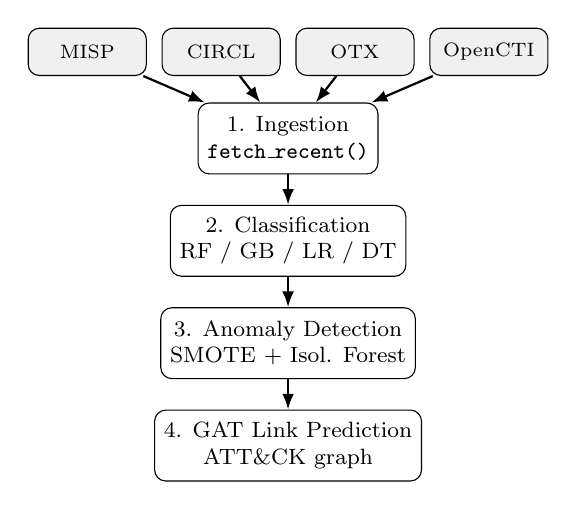
\begin{tikzpicture}[
  box/.style={draw, rounded corners, minimum width=2.1cm, minimum height=0.9cm, align=center, font=\footnotesize},
  conn/.style={draw, rounded corners, minimum width=1.5cm, minimum height=0.6cm, align=center, font=\scriptsize, fill=gray!12},
  arr/.style={-{Latex[length=2mm]}, thick}
]
\node[conn] (misp) at (0,2.1) {MISP};
\node[conn] (circl) at (1.7,2.1) {CIRCL};
\node[conn] (otx) at (3.4,2.1) {OTX};
\node[conn] (opencti) at (5.1,2.1) {OpenCTI};

\node[box] (ingest) at (2.55,1) {1. Ingestion\\ \texttt{fetch\_recent()}};
\node[box] (classify) at (2.55,-0.3) {2. Classification\\ RF / GB / LR / DT};
\node[box] (anomaly) at (2.55,-1.6) {3. Anomaly Detection\\ SMOTE + Isol. Forest};
\node[box] (gat) at (2.55,-2.9) {4. GAT Link Prediction\\ ATT\&CK graph};

\draw[arr] (misp) -- (ingest);
\draw[arr] (circl) -- (ingest);
\draw[arr] (otx) -- (ingest);
\draw[arr] (opencti) -- (ingest);
\draw[arr] (ingest) -- (classify);
\draw[arr] (classify) -- (anomaly);
\draw[arr] (anomaly) -- (gat);
\end{tikzpicture}
\caption{Four-stage pipeline and conceptual framework. All four connectors implement an identical \texttt{fetch\_recent(limit)} interface (\S\ref{sec:connector-interface}), so Stage~1 is written once against the interface, independent of source.}
\label{fig:pipeline}
\end{figure}

\begin{enumerate}
\item \textbf{Ingestion.} For each configured source, \texttt{fetch\_recent(limit)} is invoked; results are pooled with a configurable quantity of labeled synthetic data (explicitly flagged \texttt{is\_synthetic=True}) to reach a target training-set size.
\item \textbf{Classification.} Text fields are vectorized (TF-IDF) and four classifiers \textemdash{} Random Forest, Gradient Boosting, Logistic Regression, and Decision Tree \textemdash{} are trained and evaluated with a held-out test split and 5-fold cross-validation. An \emph{overfitting gate} flags any model whose train/test F1 gap exceeds 0.10 as \texttt{FAIL-overfitting}.
\item \textbf{Anomaly detection.} A SMOTE-balanced Isolation Forest \cite{liu2008isolationforest,chawla2002smote} identifies IoCs that deviate from the bulk distribution of ingested records, surfacing candidates for novel or under-represented threat patterns that a supervised classifier trained on known labels may miss.
\item \textbf{Graph link prediction.} A Graph Attention Network is trained on a MITRE ATT\&CK-derived graph of entities (threat groups, techniques, software) and their relationships, to predict plausible but unobserved technique associations.
\end{enumerate}

\subsection{Graph Attention Network Formulation}
\label{sec:gat-formulation}
Following \cite{velickovic2018gat}, node representations are updated by attending over each node's neighborhood. For node $i$ with neighborhood $\mathcal{N}(i)$, an attention coefficient over neighbor $j$ is computed as
\begin{equation}
\alpha_{ij} = \frac{\exp\left(\mathrm{LeakyReLU}\left(\mathbf{a}^{\top}[\mathbf{W}h_i \,\Vert\, \mathbf{W}h_j]\right)\right)}
{\sum_{k \in \mathcal{N}(i)} \exp\left(\mathrm{LeakyReLU}\left(\mathbf{a}^{\top}[\mathbf{W}h_i \,\Vert\, \mathbf{W}h_k]\right)\right)}
\end{equation}
where $h_i$ is node $i$'s feature vector, $\mathbf{W}$ a learned linear transform, $\mathbf{a}$ a learned attention vector, and $\Vert$ concatenation. The updated representation is $h_i' = \sigma\left(\sum_{j \in \mathcal{N}(i)} \alpha_{ij} \mathbf{W} h_j\right)$. ThreatIQ's implementation (\texttt{app/ml/gat.py}) is written in NumPy rather than a deep-learning framework, using Bellman-style iterative weight updates rather than autograd-based backpropagation. This is a deliberate engineering trade-off addressing RQ2: it removes a heavyweight GPU-oriented dependency (\texttt{torch}, \texttt{torch\_geometric}) from the default deployment path, at the cost of the training-efficiency and expressiveness advantages a framework-backed implementation would offer at larger graph scale. Link-prediction quality is reported using Hits@$k$ and Mean Reciprocal Rank (MRR), standard metrics in the knowledge-graph and information-retrieval literature (Table~\ref{tab:definitions}).

\subsection{Security Architecture}
\label{sec:security}
\textbf{Authentication.} Login issues a JWT \cite{rfc7519} bearer token (24-hour expiry) carrying subject, tenant, role, and a maximum-TLP claim. Passwords are hashed with PBKDF2-SHA256 \cite{rfc8018} at 260{,}000 iterations \textemdash{} a deliberately expensive, brute-force-resistant configuration.

\textbf{Authorization.} Three roles (\texttt{admin}, \texttt{analyst}, \texttt{viewer}) gate access to state-changing and computationally expensive routes (e.g., GAT retraining and manual connector fetches are \texttt{admin}-only).

\textbf{Data-sensitivity filtering.} Every IoC record carries a TLP label; every authenticated principal carries a maximum-TLP claim, and record access is denied (HTTP 403) when a record's TLP exceeds the caller's ceiling, independent of role.

\textbf{Rate limiting.} A token-bucket limiter, keyed by client IP address, caps default traffic at 120 requests/minute and computationally expensive routes (pipeline execution, GAT retraining, connector fetch, evaluation) at 20 requests/minute.

\subsection{Unit of Analysis and Study Object}
Because this is artifact-evaluation research (\S\ref{sec:framework}), the unit of analysis is the ThreatIQ v4.0 software system itself, deployed on a single-node, single-worker evaluation environment (\S\ref{sec:evaluation}), not a human population. Accordingly, there are no human respondents, no survey or interview instruments, and no probability sampling of participants; the closest analogue to ``study area and respondents'' in a conventional empirical study is the specific, fully disclosed software and hardware configuration under which every measurement in Section~\ref{sec:evaluation} was taken.

\subsection{Test Data Configuration (Sampling Analogue)}
\label{sec:sampling}
Where a conventional empirical study would describe sampling technique and sample size, this study reports its analogous \emph{test data configuration}: (i) a classification/anomaly-detection pool of $n=800$ records (12 live/offline-sample connector records pooled with 788 labeled synthetic records; \S\ref{sec:evaluation}); (ii) a GAT evaluation set of 2--4 held-out relationship pairs drawn from an offline MITRE ATT\&CK relationship sample (\S\ref{sec:evaluation}); and (iii) two load-testing configurations of 15 and 20 concurrent simulated users (\S\ref{sec:loadtest}). None of these involve probability sampling from a human population; all three are fully specified and reproducible from the parameters given.

\subsection{Data Sources}
\textbf{Primary data} consist of artifacts produced by executing the live system: HTTP responses, application logs (via \texttt{structlog}), pytest results, and Locust load-test statistics. \textbf{Secondary data} consist of the MITRE ATT\&CK relationship corpus \cite{strom2018attack} and the STIX 2.1 specification \cite{stix21} used to structure the GAT's input graph and the OpenCTI connector's output format, respectively.

\subsection{Data Collection Procedure}
Data were collected in three passes: (1) a clean dependency installation followed by automated test execution (\texttt{pytest}), producing pass/fail and timing data; (2) a live pipeline run against a running Uvicorn instance, producing classifier, anomaly-detection, and GAT metrics together with application logs used to root-cause defects (\S\ref{sec:implementation}); and (3) two Locust-driven concurrent load tests at increasing simulated-user counts, producing per-route latency and status-code distributions (\S\ref{sec:loadtest}).

\subsection{Instruments}
\label{sec:instruments}
Consistent with DSR artifact-evaluation practice, this study's ``instruments'' are software tools rather than survey or interview guides: \texttt{pytest} (56 automated test cases spanning security primitives, all four connectors, the GAT trainer, and two end-to-end pipeline-integration tests), Locust (concurrent HTTP load generation with role-weighted, authenticated traffic), \texttt{curl}/\texttt{httpx} (manual endpoint verification), and \texttt{structlog}-based application logging (defect root-causing).

\subsection{Data Analysis Procedure}
Classification quality is analyzed via test-set F1, AUC, Matthews Correlation Coefficient (MCC), 5-fold cross-validated F1, and the train/test F1 gap (the overfitting-gate statistic). Anomaly-detection quality is analyzed via precision, recall, and F1 on the anomaly-labeled subset. GAT quality is analyzed via Hits@$k$ ($k \in \{1,5,10\}$) and MRR on a held-out relationship split. Load-test data are analyzed via per-route median and p95 latency and HTTP status-code distribution, with failure causes root-caused individually (\S\ref{sec:findings}) rather than reported as an undifferentiated failure rate.

\subsection{Ethical Considerations}
\label{sec:ethics}
This study involves no human participants, no personally identifiable information, and no vulnerable populations; formal human-subjects ethics review is therefore not applicable, consistent with standard practice for artifact-evaluation design-science research \cite{hevner2004design}. Three considerations remain relevant and are addressed explicitly. \textbf{Authorized access}: live testing of the OTX connector used only the researcher's own free-tier, self-service API credentials, obtained and used in compliance with the provider's terms of service; no unauthorized access, credential sharing, or scraping was performed. \textbf{Responsible disclosure}: three pre-existing defects in the evaluated codebase (\S\ref{sec:implementation}) were identified, root-caused, and corrected within this same body of work rather than disclosed publicly without remediation or exploited. \textbf{Data provenance}: evaluation data are either synthetic (explicitly flagged \texttt{is\_synthetic=True}) or drawn from connectors' own offline-fallback samples and public pulse data; no proprietary or confidential third-party data were used.

%======================================================================
\section{Implementation and Reproducibility Engineering}
\label{sec:implementation}
%======================================================================

Beyond the connector substitution itself, live end-to-end execution of the platform (rather than static review alone) surfaced defects that a conventional unit-test suite did not catch, because each requires either a full dependency-resolution pass or a running, stateful pipeline to observe. We report these because we believe under-reporting of \emph{reproducibility} defects in applied-systems papers understates a real cost of operating CTI tooling, and because they constitute direct evidence for RQ3 (\S\ref{sec:questions}) and design proposition DP2 (\S\ref{sec:propositions}).

\begin{enumerate}
\item \textbf{Unresolvable dependency pin.} The dependency manifest pinned \texttt{taxii2-client==2020.4.21}, a version string that does not correspond to any release published to the Python Package Index; the newest available release at the time of this study was \texttt{2.3.0}. A clean installation from the manifest therefore failed unconditionally, before any application code executed.
\item \textbf{Missing transitive dependencies.} The authentication module imports \texttt{python-jose} and \texttt{passlib} (with a \texttt{bcrypt} backend) directly, but neither package was declared in the dependency manifest. A clean install (once the pin above is corrected) would install successfully but fail at import time on application startup.
\item \textbf{Unserializable response type.} The pipeline-status endpoint computed an overfitting flag as \texttt{gap > 0.10}, where \texttt{gap} is a \texttt{numpy.float64} produced by a scikit-learn F1-score computation; the comparison yields a \texttt{numpy.bool\_}, a type the API framework's JSON serializer cannot encode. Every call to the status endpoint following a completed pipeline run therefore raised an unhandled server error. This defect was present in exactly one of two structurally identical call sites in the codebase (the evaluation endpoint's equivalent computation was already correctly wrapped in a native \texttt{bool()} cast), illustrating how such defects can persist even in code with an established, correct pattern elsewhere in the same file.
\end{enumerate}

All three were identified by executing the application \textemdash{} a clean dependency install followed by a live pipeline run \textemdash{} rather than by code reading, and all three are corrected in the version evaluated in Section~\ref{sec:evaluation}.

%======================================================================
\section{Results and Evaluation}
\label{sec:evaluation}
%======================================================================

All results in this section were obtained by executing the live application (not simulated or estimated) on a single-node sandboxed evaluation environment: Python 3.12.3, single Uvicorn worker process, in-memory route handlers (see \S\ref{sec:threats} for the persistence-layer caveat), no GPU.

\subsection{Correctness Testing}
The automated test suite (56 cases, covering security primitives, all four connectors, the GAT trainer, the reinforcement-learning feedback agent, the OpenCTI enrichment path, and two end-to-end pipeline-integration tests) passed at 56/56 (100\%) in 23.4\,s on a clean, freshly provisioned virtual environment, confirming both correctness and that the dependency-manifest fixes described in \S\ref{sec:implementation} resolve the installation defect rather than merely working around it in a pre-patched environment.

\subsection{Classification and Anomaly Detection}
A full pipeline run ingested 12 live/offline-sample records across the MISP, CIRCL, and OTX connectors (5, 3, and 4 records respectively, each source's offline-fallback path, since no production API credentials were configured for this evaluation run) pooled with 788 synthetic records for a target size of 800. Table~\ref{tab:classification} reports the four-classifier comparison; all four pass the overfitting gate ($\mathrm{gap} \leq 0.10$).

\begin{table}[h]
\caption{Classification results, $n=800$ (12 real/offline-sample + 788 synthetic)}
\label{tab:classification}
\centering
\begin{tabular}{@{}lccccc@{}}
\toprule
\textbf{Model} & \textbf{Test F1} & \textbf{AUC} & \textbf{MCC} & \textbf{Gap} & \textbf{CV F1} \\
\midrule
Random Forest & 0.957 & 0.998 & 0.950 & 0.001 & 0.924 \\
Gradient Boosting & 0.988 & 1.000 & 0.986 & 0.009 & 0.959 \\
Logistic Regression & 0.932 & 0.987 & 0.921 & $-$0.016 & 0.910 \\
Decision Tree & 0.845 & 0.969 & 0.830 & 0.030 & 0.824 \\
\bottomrule
\end{tabular}
\end{table}

The SMOTE-balanced Isolation Forest anomaly detector achieved precision 0.40, recall 0.50, and F1 0.444 against the anomaly-labeled subset of the same run. We report this without embellishment: at this sample size and with a heavily synthetic-dominated pool, this metric should be read as a pipeline-validity check (the anomaly stage executes correctly and produces a coherent precision/recall trade-off) rather than a claim about real-world anomaly-detection performance, which would require a larger, more label-diverse evaluation set (\S\ref{sec:threats}).

\subsection{GAT Link Prediction}
The GAT was trained for 200 epochs on the platform's offline MITRE ATT\&CK relationship sample (used because no production STIX bundle was downloaded into the evaluation environment; see \S\ref{sec:threats}), reaching a final training loss of 53.48. Table~\ref{tab:gat} reports link-prediction quality on the held-out test split, addressing RQ2 and design proposition DP3.

\begin{table}[h]
\caption{GAT link-prediction metrics (200 epochs, offline ATT\&CK sample)}
\label{tab:gat}
\centering
\begin{tabular}{@{}lcccc@{}}
\toprule
\textbf{Split} & \textbf{Hits@1} & \textbf{Hits@5} & \textbf{Hits@10} & \textbf{MRR} \\
\midrule
Full evaluation ($n=4$ pairs) & 0.250 & 1.000 & 1.000 & 0.425 \\
Held-out test ($n=2$ pairs) & 0.500 & 1.000 & 1.000 & 0.750 \\
\bottomrule
\end{tabular}
\end{table}

\textbf{We flag this explicitly as a low-statistical-power result}: with only 2--4 evaluation pairs, Hits@5 and Hits@10 saturating at 1.000 is close to trivially achievable and should not be read as evidence of strong generalization. We report it transparently as a pipeline-correctness demonstration (the GAT trains, converges, saves, reloads, and produces well-formed ranked predictions end-to-end) and explicitly identify benchmark-scale evaluation against the full MITRE ATT\&CK STIX corpus as required future work (\S\ref{sec:future}).

\subsection{Load Testing}
\label{sec:loadtest}
We used Locust to drive concurrent, role-weighted synthetic traffic against every documented API route, authenticating as a weighted mix of the three roles and issuing role-appropriate request bodies. Table~\ref{tab:loadtest} compares two runs at increasing concurrency.

\begin{table}[h]
\caption{Load test summary at two concurrency levels}
\label{tab:loadtest}
\centering
\begin{tabular}{@{}lcc@{}}
\toprule
 & \textbf{Run A (light)} & \textbf{Run B (heavier)} \\
\midrule
Simulated users & 15 & 20 \\
Duration & 25 s & 40 s \\
Total requests & 98 & 194 \\
Failed requests & 0 (0\%) & 47 (24.2\%) \\
Median latency (all routes) & $<$10 ms & 4 ms \\
p95 latency (all routes) & $<$50 ms & 10{,}000 ms \\
\bottomrule
\end{tabular}
\end{table}

\subsection{Findings from Load Testing}
\label{sec:findings}
Run B's elevated failure rate and tail latency are attributable to two distinct, identifiable causes rather than generic instability, directly answering RQ3:

\textbf{(1) Rate-limiter IP-keying under single-origin load.} All 47 failures in Run B carried HTTP 429 (Too Many Requests). The platform's rate limiter is keyed by client IP address rather than by authenticated principal (\S\ref{sec:security}); because all 20 simulated users in a Locust run originate from a single test-harness IP, they collectively share one token bucket. This is a correct, intentional behavior of an IP-keyed limiter defending against a single high-volume source, but it means that single-origin load testing systematically under-represents the concurrency a real multi-tenant deployment (with distinct client IPs per organization or egress gateway) could sustain before triggering the same limiter. We report this as an evaluation-methodology caveat as much as a system finding.

\textbf{(2) Synchronous password hashing blocking the async event loop.} The authentication route's PBKDF2-SHA256 hashing (\S\ref{sec:security}) is CPU-bound and, in the evaluated build, invoked synchronously within an \texttt{async def} route handler. Under FastAPI/Uvicorn's single-worker, single-event-loop execution model, a CPU-bound synchronous call blocks the loop for its full duration, serializing concurrent requests rather than interleaving their I/O-bound portions. At 18 concurrent login attempts (Run B), \texttt{POST /api/v1/auth/login} showed a median latency near 10 seconds and a maximum near 11.8 seconds \textemdash{} substantially higher than any other route, all of which are dominated by I/O rather than CPU-bound cryptographic work. This is a specific, actionable finding: moving the hashing call to a thread-pool executor (e.g., via \texttt{run\_in\_executor}) or a dedicated worker pool would be expected to remove this bottleneck without weakening the hashing configuration itself, since the 260{,}000-iteration cost is a deliberate security parameter, not an accidental one.

We consider both findings a demonstration of the value of live, concurrent execution as an evaluation method for CTI platforms: neither is visible from the unit test suite, and (1) in particular would not be visible from a single-user functional smoke test regardless of realism, since it is inherently a property of concurrent, single-origin access.

%======================================================================
\section{Discussion}
%======================================================================

\subsection{Synthesis Against Research Questions}
RQ1 is answered affirmatively for the evaluated case: the connector interface (\S\ref{sec:connector-interface}) allowed FS-ISAC to be replaced by OTX with zero downstream code changes (\S\ref{sec:migration}). RQ2 is partially answered: the NumPy-only GAT completes a full train\textendash evaluate\textendash predict cycle without a GPU (\S\ref{sec:evaluation}), but the accuracy/resource trade-off relative to a framework-backed baseline remains unquantified at this evaluation's scale (\S\ref{sec:threats}) and is identified as future work (\S\ref{sec:future}). RQ3 is answered with two concrete, root-caused findings (\S\ref{sec:findings}) plus three reproducibility defects (\S\ref{sec:implementation}), all invisible to the pre-existing unit-test suite.

\subsection{Limitations and Threats to Validity}
\label{sec:threats}

\textbf{Evaluation scale.} The classification and anomaly-detection results (\S\ref{sec:evaluation}) were obtained on a pool dominated by synthetic data (788 of 800 records) supplemented by a small number of connector offline-fallback samples, because production API credentials for MISP, CIRCL, and OTX were not provisioned in the evaluation environment. The reported metrics validate pipeline correctness and the overfitting-gate mechanism, not real-world classification accuracy on live threat feeds; a production evaluation should report metrics computed exclusively on the \texttt{is\_synthetic=False} subset at a scale of thousands of live-sourced records.

\textbf{GAT statistical power.} As flagged in \S\ref{sec:evaluation}, the GAT link-prediction evaluation used 2--4 held-out pairs from an offline ATT\&CK relationship sample, not the full downloaded MITRE ATT\&CK STIX corpus (the corpus was not present in the evaluation environment's \texttt{data/} directory). Hits@$k$ metrics at this sample size have wide, unreported confidence intervals and should not be compared against benchmark-scale GNN literature results.

\textbf{Persistence layer.} PostgreSQL and the corresponding SQLAlchemy schema are present in the codebase and start successfully under the containerized deployment, but the evaluated API route handlers use in-process, non-persistent mock data rather than the database; consequently, the load-testing results in \S\ref{sec:loadtest} characterize the application and connector layers under concurrency, not database-backed persistence under concurrency, which is a materially different (and currently unmeasured) evaluation.

\textbf{Single-node, single-worker deployment.} All live measurements were taken against a single Uvicorn worker process on a single node. Production deployments typically run multiple worker processes behind a load balancer, which would change both the rate-limiter's effective capacity (unless centralized, e.g., via Redis) and the severity of the synchronous-hashing bottleneck (\S\ref{sec:findings}), since concurrent requests would be distributed across independent event loops rather than serialized on one.

\textbf{Single-origin load generation.} As discussed in \S\ref{sec:findings}, Locust-driven load in this study originated from a single client IP, which interacts specifically with the platform's IP-keyed rate limiter in a way that would not generalize directly to a distributed, multi-tenant traffic pattern.

%======================================================================
\section{Extension: SIEM Integration and Standards Interoperability}
\label{sec:extension}
%======================================================================
The sections above report the system and evaluation as originally submitted. This section reports a subsequent extension pass, applying the same live-verification methodology (\S\ref{sec:instruments}) to a distinct set of engineering additions rather than revising the original evaluation's numbers. We separate this material into its own section, rather than folding it into \S\ref{sec:evaluation}, so that the original, submitted results remain independently reproducible from the artifact accompanying this paper.

\subsection{Motivation}
The original architecture (\S\ref{sec:architecture}) treats CTI feeds purely as ingestion sources and MITRE ATT\&CK purely as a training substrate for the GAT. Two practitioner-facing gaps follow from this scope. First, a CTI platform that only ingests and classifies, without feeding a security operations team's actual detection surface (a SIEM), stops short of the point where classification becomes an operational action. Second, exporting enrichment only through a MISP-shaped connector (\S\ref{sec:litreview}) ties interoperability to one specific platform, when the wider field has converged on vendor-neutral standards (STIX 2.1 \cite{stix21} for indicators, the MITRE ATT\&CK Navigator layer format for technique coverage) that a broader set of tools can consume directly.

\subsection{Audit Findings Predating the Extension}
\label{sec:extension-audit}
Before adding new functionality, the codebase was audited directly (not simply re-read from documentation). This audit found a live-looking API key hardcoded as the default value of a configuration field, already committed to version-control history, meaning every clone of the repository carried a working credential by default. This is a distinct finding from the live-execution defects reported in \S\ref{sec:implementation}: it was located by static inspection, not live execution, and it is reported here for the same reason those defects were reported there \textemdash{} under-reporting operationally relevant findings, whatever method locates them, understates the real cost of operating CTI tooling. The key was invalidated and the default removed. The same audit also located and removed an accidental, fully duplicated nested copy of the entire project directory tree, which had been committed to version control and roughly doubled repository size for no functional reason.

\subsection{Bidirectional SIEM Integration}
A new connector, structurally identical to the existing MISP/CIRCL/OTX connectors (same \texttt{fetch\_recent(limit) -> list[dict]} interface, same offline-fallback contract; \S\ref{sec:connector-interface}), treats a Wazuh SIEM deployment as another CTI source: alerts at or above a minimum rule severity are queried from Wazuh's OpenSearch-compatible indexer API and normalized into ThreatIQ's standard IoC schema. This is a direct, additional test of DP1 (\S\ref{sec:propositions}): the connector interface again permitted a structurally different upstream system (a SIEM's alert store, rather than a CTI feed) to be added with zero changes to the classification, GAT, or API-routing layers.

The reverse direction \textemdash{} publishing ThreatIQ's own output \textemdash{} required a new component, since no existing connector pushes data outward. A MISP-export module filters classified indicators by confidence and severity threshold, excludes synthetic training records, and publishes qualifying indicators as a MISP Event. A SIEM's own MISP integration (external to ThreatIQ, configured on the SIEM side) can then poll that event and auto-generate detection rules from it. This closes a loop that the original architecture left open: CTI sources feed ThreatIQ, ThreatIQ's classification feeds a SIEM's detection surface, and the SIEM's resulting alerts feed back into ThreatIQ as a new CTI source via the same pull-direction connector.

\subsection{Open-Standards Interoperability}
Two export services were added, both deliberately standalone (no dependency on the MISP-specific export path above), so that ThreatIQ's classification output is consumable without ThreatIQ or MISP present at all. A STIX 2.1 export service converts IoC records into a standards-compliant Bundle: indicator IDs are generated as UUIDv5 values deterministically derived from the indicator value, so re-exporting the same indicator across pipeline runs yields the same object identity (idempotent republication) rather than a duplicate; confidence values are converted from ThreatIQ's internal $[0,1]$ scale to the integer $[0,100]$ scale the STIX 2.1 specification requires; indicator types with no corresponding STIX Cyber Observable Object (e.g., a bare hostname) are exported as an annotation-only Note rather than mapped onto a fabricated observable type, to avoid a false claim of standards compliance. A second service converts the GAT's \texttt{(actor, technique, score)} predictions (\S\ref{sec:gat-formulation}) into a MITRE ATT\&CK Navigator layer file, resolving each prediction's technique name back to its canonical technique ID and taking the maximum predicted score across contributing actors per technique (rather than summing or averaging) so that a technique predicted likely by several distinct actors is not diluted relative to one predicted by a single actor with equal confidence.

\subsection{Cross-Source Correlation}
A correlation service groups IoC records by normalized \texttt{(value, type)} pair across all connectors and merges records that independently agree on the same observable, boosting the merged record's confidence in proportion to the number of distinct corroborating sources (capped, and applied multiplicatively against the remaining headroom to $1.0$ rather than as a flat additive bonus, so that volume of low-quality corroboration cannot alone drive confidence to its ceiling). This operationalizes, at the level of individual indicators, the same reliability/credibility separation underlying the Admiralty (NATO) system of source grading used in traditional intelligence tradecraft: agreement between independent sources is treated as evidence in its own right, not merely as additional volume. This mechanism is deliberately exposed as a separate, explicitly-invoked endpoint rather than folded into the default pipeline (\S\ref{sec:methodology}), because it changes indicator \emph{counts} by merging duplicates, and the pipeline's classifier/GAT metrics reported in \S\ref{sec:evaluation} are numbers this paper commits to as reproducible from the accompanying artifact.

\subsection{Verification of the Extension}
\label{sec:extension-verification}
The same verification discipline argued for in \S\ref{sec:implementation}--\S\ref{sec:findings} was applied to this extension. The automated test suite grew from 56 to 100 cases (44 new: connector/exporter behavior, STIX/Navigator conversion correctness, and correlation semantics), all passing. Beyond unit tests, every new HTTP endpoint was exercised against a live running instance with real authenticated requests under all three role tokens (admin, analyst, viewer), confirming both correct-case behavior and role-based-access-control enforcement (e.g., a viewer token correctly receives HTTP 403 on the correlation endpoint). A full pipeline run with the new SIEM source included in the source list was executed end-to-end and ingested alerts from the new connector alongside the three original sources, with all classifiers continuing to pass the overfitting gate. Because an earlier verification step in this same pass exercised GAT retraining and therefore overwrote the trained-weights artifact underlying Table~\ref{tab:gat}, that artifact was explicitly restored from version control before concluding the pass, so the GAT metrics reported in \S\ref{sec:evaluation} remain reproducible from the accompanying artifact exactly as originally evaluated.

\subsection{Scope Limitations of the Extension}
This extension was verified against each connector's offline-fallback mode; no live Wazuh deployment or live MISP instance was available in the evaluation environment, so the live-mode code paths for both the SIEM connector and the MISP-export module are exercised by unit tests with mocked/unreachable endpoints (confirming graceful fallback) rather than by a live external system. Correlation across the fully offline demonstration data shows zero cross-source corroboration, because each connector's offline sample set was authored independently and none happen to share a literal indicator value; this is the expected, correct behavior of the correlation logic given that input, not a defect, and real corroboration is only exercised once at least two connectors are live against overlapping real-world infrastructure. Similarly, the ATT\&CK Navigator export frequently returns zero techniques against the currently trained GAT weights, for the same reason already reported in \S\ref{sec:threats}: the offline MITRE relationship sample is small enough that few predicted links clear the model's confidence threshold. Both limitations are direct consequences of evaluation-environment scale already disclosed in \S\ref{sec:threats}, not new limitations introduced by this extension.

%======================================================================
\section{Future Work}
\label{sec:future}
%======================================================================
Four directions would most directly strengthen this work toward a more rigorous, benchmark-comparable evaluation: (1) provisioning live production credentials for all four connectors and reporting classification/anomaly metrics exclusively on live-sourced data at production scale; (2) downloading and training against the full MITRE ATT\&CK enterprise STIX corpus, reporting Hits@$k$/MRR with confidence intervals and a comparison against a \texttt{torch\_geometric}-based GAT baseline to quantify the NumPy implementation's accuracy/efficiency trade-off (directly closing the RQ2 gap identified in \S\ref{sec:threats}); (3) wiring the existing SQLAlchemy persistence layer into the API route handlers and repeating the load-testing methodology of \S\ref{sec:loadtest} against database-backed state; and (4) distributed, multi-origin load generation to characterize the rate limiter and the concurrency bottleneck identified in \S\ref{sec:findings} under conditions closer to a real multi-tenant deployment. A fifth direction follows directly from \S\ref{sec:extension}: standing up a live Wazuh deployment and a live MISP instance to exercise the SIEM integration's live-mode code paths end-to-end, and repeating the correlation and Navigator-export evaluations against real, overlapping multi-source data rather than independently-authored offline samples, which is the specific condition under which both mechanisms are expected to produce non-trivial output.

%======================================================================
\section{Conclusion}
%======================================================================
We presented ThreatIQ v4.0, an applied CTI aggregation platform built around a uniform, connector-agnostic ingestion interface, a classical-ML triage pipeline with an explicit overfitting gate, a dependency-minimal GAT for MITRE ATT\&CK link prediction, and a defense-in-depth API security layer. Framed within the design-science research paradigm \cite{hevner2004design}, we used a concrete connector-substitution case study (FS-ISAC $\rightarrow$ OTX) to evaluate design proposition DP1 and answer RQ1, and we reported a live-verification methodology \textemdash{} full pipeline execution and concurrent load testing, not unit testing alone \textemdash{} that evaluated DP2 and answered RQ3 by surfacing and allowing us to fix a dependency-resolution defect, an import-time defect, a JSON-serialization defect, and by characterizing a genuine concurrency bottleneck in synchronous password hashing under an asynchronous serving model. In a subsequent extension (\S\ref{sec:extension}), the same connector-agnostic pattern and live-verification discipline were applied again to add a bidirectional SIEM integration, open-standards (STIX 2.1, ATT\&CK Navigator) export, and cross-source correlation, evaluating design proposition DP4 and, in the course of that work, surfacing and remediating a hardcoded-credential exposure that static audit \textemdash{} independent of the live-execution methodology used elsewhere in this paper \textemdash{} was needed to catch. We reported all quantitative results transparently, including their sample-size and scale limitations, and outlined the specific steps required to extend this evaluation to production scale and fully answer RQ2. We believe the connector-interface pattern, the live-verification methodology, and the honestly-scoped evaluation reporting are each independently useful to practitioners and researchers building or assessing CTI tooling, irrespective of the specific machine-learning components used.

%======================================================================
\section{Research Timeline}
\label{sec:timeline}
%======================================================================
Table~\ref{tab:timeline} summarizes the study's phase structure. Exact calendar dates are omitted from this manuscript and should be inserted by the author to match the specific submission portal's requirements, where required.

\begin{table}[h]
\caption{Research timeline by phase}
\label{tab:timeline}
\centering
\begin{tabular}{@{}p{0.6cm}p{3.0cm}p{4.0cm}@{}}
\toprule
\textbf{Phase} & \textbf{Activity} & \textbf{Primary Outputs} \\
\midrule
1 & Requirements \& architecture design & Connector interface spec, layer design (\S\ref{sec:architecture}) \\
2 & Connector implementation \& migration & OTX connector, FS-ISAC substitution (\S\ref{sec:migration}) \\
3 & Pipeline \& model implementation & Classification, anomaly detection, GAT (\S\ref{sec:methodology}) \\
4 & Live verification \& load testing & Defect reports (\S\ref{sec:implementation}), load-test data (\S\ref{sec:loadtest}) \\
5 & Analysis, writing \& dissemination & This manuscript; presentation and poster materials \\
\bottomrule
\end{tabular}
\end{table}

\section*{Acknowledgment}
The author thanks the AAA (Aroop AI Academy) and Arslan Institute of Technology (AiT) communities for context and feedback during the development of this platform, and the BUP Research Society for the structured research-roadmap guidance that informed the organization of this manuscript.

\begin{thebibliography}{00}

\bibitem{strom2018attack} B. E. Strom, A. Applebaum, D. P. Miller, K. C. Nickels, A. G. Pennington, and C. B. Thomas, ``MITRE ATT\&CK: Design and Philosophy,'' Technical Report, The MITRE Corporation, MP180360, Jul. 2018.

\bibitem{velickovic2018gat} P. Veli\v{c}kovi\'{c}, G. Cucurull, A. Casanova, A. Romero, P. Li\`{o}, and Y. Bengio, ``Graph Attention Networks,'' in \textit{Proc. Int. Conf. Learning Representations (ICLR)}, 2018.

\bibitem{liu2008isolationforest} F. T. Liu, K. M. Ting, and Z.-H. Zhou, ``Isolation Forest,'' in \textit{Proc. 8th IEEE Int. Conf. Data Mining (ICDM)}, 2008, pp. 413--422.

\bibitem{chawla2002smote} N. V. Chawla, K. W. Bowyer, L. O. Hall, and W. P. Kegelmeyer, ``SMOTE: Synthetic Minority Over-sampling Technique,'' \textit{J. Artificial Intelligence Research}, vol. 16, pp. 321--357, 2002.

\bibitem{breiman2001randomforest} L. Breiman, ``Random Forests,'' \textit{Machine Learning}, vol. 45, no. 1, pp. 5--32, 2001.

\bibitem{friedman2001gbm} J. H. Friedman, ``Greedy Function Approximation: A Gradient Boosting Machine,'' \textit{Annals of Statistics}, vol. 29, no. 5, pp. 1189--1232, 2001.

\bibitem{stix21} B. Jordan, R. Piazza, and T. Darley, ``STIX Version 2.1,'' OASIS Cyber Threat Intelligence Technical Committee Standard, Jul. 2021. [Online]. Available: https://docs.oasis-open.org/cti/stix/v2.1/stix-v2.1.html

\bibitem{nist800150} C. Johnson, L. Badger, D. Waltermire, J. Snyder, and C. Skorupka, ``Guide to Cyber Threat Information Sharing,'' NIST Special Publication 800-150, National Institute of Standards and Technology, Oct. 2016.

\bibitem{rfc7519} M. Jones, J. Bradley, and N. Sakimura, ``JSON Web Token (JWT),'' IETF RFC 7519, May 2015.

\bibitem{rfc8018} K. Moriarty, B. Kaliski, and A. Rusch, ``PKCS \#5: Password-Based Cryptography Specification Version 2.1,'' IETF RFC 8018, Jan. 2017.

\bibitem{first_tlp} FIRST.org, ``Traffic Light Protocol (TLP) Definitions and Usage,'' 2022. [Online]. Available: https://www.first.org/tlp/

\bibitem{alienvaultotx} AT\&T Cybersecurity, ``AlienVault Open Threat Exchange (OTX) API Documentation,'' 2024. [Online]. Available: https://otx.alienvault.com/api

\bibitem{hevner2004design} A. R. Hevner, S. T. March, J. Park, and S. Ram, ``Design Science in Information Systems Research,'' \textit{MIS Quarterly}, vol. 28, no. 1, pp. 75--105, 2004.

\bibitem{bgdcirt} BGD e-GOV CIRT, ``About BGD e-GOV CIRT,'' Bangladesh Computer Council, 2024. [Online]. Available: https://www.cirt.gov.bd/

\end{thebibliography}

\appendices

\section{BUP Research Roadmap Compliance Crosswalk}
\label{app:crosswalk}
Table~\ref{tab:crosswalk} maps each of the 21 components in the BUP Research Society's Research Roadmap to the section of this manuscript that addresses it, noting adaptations made for an applied systems/engineering paper rather than a primary human-subjects study.

\begin{table}[h]
\caption{Roadmap-to-manuscript crosswalk}
\label{tab:crosswalk}
\centering
\footnotesize
\begin{tabular}{@{}p{0.4cm}p{2.3cm}p{4.9cm}@{}}
\toprule
\textbf{\#} & \textbf{Roadmap Component} & \textbf{Manuscript Location / Adaptation} \\
\midrule
1 & Title & Title page \\
2 & Abstract & Abstract \\
3 & Introduction & \S I \\
4 & Background of the Study & \S I-A \\
5 & Statement of the Problem & \S I-B \\
6 & Literature Review & \S II \\
6.1 & Research Gap & \S II-E \\
7 & Research Questions & \S III \\
8 & Research Objectives & \S I-E \\
9 & Hypotheses & \S IV-B (adapted to \emph{design propositions}, the DSR analogue of hypotheses for artifact-evaluation research \cite{hevner2004design}) \\
10 & Theoretical Framework & \S IV-A \\
11 & Conceptual Framework & \S IV-C, Fig.~1 \\
12 & Rationale of the Study & \S I-C \\
13 & Significance of the Study & \S I-D \\
14 & Research Methodology & \S V \\
14.1--14.2 & Philosophy \& Approach & \S V-A, V-B \\
14.3 & Design & \S V-C \\
14.3.1 & Method & Mixed: quantitative metrics + qualitative defect analysis (\S V-M) \\
14.3.2 & Study Area \& Respondents & \S V-G (adapted: unit of analysis is the software artifact; no human respondents) \\
14.3.3 & Sampling & \S V-H (adapted: test-data configuration) \\
14.3.4 & Data Sources & \S V-I \\
14.3.5 & Data Collection & \S V-J \\
14.3.6 & Instruments & \S V-K (adapted: software tools, not survey instruments) \\
14.3.7 & Data Analysis & \S V-L \\
15 & Ethical Considerations & \S V-M \\
16 & Scope \& Limitations & \S I-F (scope); \S VIII-B (limitations) \\
17 & Definitions of Key Terms & \S I-F, Table~I \\
18 & Tentative Chapter Outline & Not applicable \textemdash{} this manuscript uses a continuous IEEE section structure rather than thesis chapters; the section list (this table) is the structural equivalent \\
19 & Timeline & \S XII \\
20 & Referencing & IEEE numbered style is retained throughout, rather than Harvard/APA, to comply with the target publication venue's own house style; see Author's Note below \\
21 & Appendices & Appendix A (this table), Appendix B \\
\bottomrule
\end{tabular}
\end{table}

\textit{Author's Note on Referencing Style.} The BUP Research Roadmap recommends Harvard/APA referencing for general research reports. This manuscript instead retains IEEE numbered citation style throughout, because it is formatted for IEEE-style venues, where IEEE referencing is the mandatory house style. Authors adapting this manuscript for an APA/Harvard-referencing venue should convert the bibliography accordingly; the underlying source list does not change.

\section{Supplementary Technical Detail: API Surface}
\label{app:api}
Table~\ref{tab:api} summarizes the primary API routes exercised during the original evaluation (\S\ref{sec:evaluation}) and the extension (\S\ref{sec:extension}), provided for reproducibility. All routes are prefixed with \texttt{/api/v1} (omitted below for column width). Routes below the midrule were added in the extension.

\begin{table}[h]
\caption{Primary API routes exercised during evaluation}
\label{tab:api}
\centering
\footnotesize
\begin{tabular}{@{}p{1.0cm}p{4.0cm}p{2.2cm}@{}}
\toprule
\textbf{Method} & \textbf{Route (relative to \texttt{/api/v1})} & \textbf{Purpose} \\
\midrule
POST & \texttt{/auth/login} & Issue JWT token \\
GET & \texttt{/connectors} & Connector status \\
POST & \texttt{/connectors/\{name\}/\allowbreak fetch} & Manual fetch (admin) \\
POST & \texttt{/pipeline/run} & Trigger pipeline \\
GET & \texttt{/pipeline/status} & Poll run status \\
POST & \texttt{/graph/train} & Retrain GAT (admin) \\
POST & \texttt{/evaluation/run} & Run evaluation \\
GET & \texttt{/evaluation/gat} & Get GAT Hits@$k$/MRR \\
\midrule
POST & \texttt{/connectors/\allowbreak correlate} & Cross-source correlation (admin/analyst) \\
POST & \texttt{/connectors/\allowbreak misp/export} & Publish classified IoCs to MISP (admin) \\
GET & \texttt{/iocs/\allowbreak export/stix} & Export IoCs as a STIX 2.1 bundle \\
GET & \texttt{/graph/\allowbreak navigator-layer} & Export GAT predictions as an ATT\&CK Navigator layer \\
\bottomrule
\end{tabular}
\end{table}

\end{document}
